\section{Approach}
\label{sec:approach}
% In this section, we presented the pipeline of our two experiments\MY{We never mentioned the two experiments in previous text. I rewrite: In this section, we detail our method on social media data collection and analysis~(Sec.\ref{sec:collect_data}). A two-stage proactive interaction pipeline is further proposed: we first identify designated users and select posts as ice-breaking candidates~(Sec.\ref{sec:depression_detection}); then we initiate a ``three-round interaction''~(Sec.\ref{sec:3round}) which constitutes \textbf{R1} User post, \textbf{R2} chatbot icebreaking reply, and \textbf{R3} User reply} %~\figref{fig:pipeline1} shows the selection of target users and target posts, and ~\figref{fig:pipeline2} shows the three rounds of interaction between robots or humans and depressed users, and provide some technical details. 
In this section, we provide a detailed description of our method for social media data collection and analysis~(Sec.\ref{sec:collect_data}). Additionally, we propose a two-stage proactive interaction pipeline: first, we identify targeted users and select posts as ice-breaking candidates~(Sec.\ref{sec:depression_detection}); then we initiate a \textbf{``Three-Round Interaction''}~(Sec.\ref{sec:3round}), consisting of three steps: \textbf{R1} Identification of Post for Ice-breaking, \textbf{R2} Icebreaker Generation, and \textbf{R3} User response.

%\KZ{Re-arrange this pic to make it flatter and save some space.}
%\KZ{There's some problem with this overview. I think you need to include ``interaction'' with the user,
%and specifically, we need to indicate the last three %rounds of conversation clearly, that is,
%user post, bot reply, and user response. And then we do %analysis on the result again. Now it seems that
%analysis is only done on the user posts. But actually %that's not the case right?}

\subsection{Depression Data Collection}
\label{sec:collect_data}
%In this work, we collect data from weibo, which is a social media platform widely used 
%by Chinese Internet users- contains a large group of people from all walks of life, 
%and each user’s emotional state can be expressed by his posts on Weibo.
Existing research primarily focuses on using Twitter or Facebook to study depression~\cite{sadeque2018measuring}, which overlooks the large depressive population in China, as these platforms are blocked in mainland China. By contrast, Sina Weibo\footnote{https://m.weibo.cn/} (hereafter referred to as Weibo) is the most popular social media platform in China and is considered the Chinese equivalent of X (formerly Twitter). It has over 500 million registered users from diverse backgrounds and generates more than 100 million microblogs daily.

%We use a depressed users detector to monitor the Depression Super Topic Community on Weibo.
%We use our proactive ice-breaking system\MY{what is the system? it seem the system is referring to many things. I think here it's the depressive user detector? please be specific} to monitor the users who have posted in 
%Weibo Depression Super Topic Community. 
%The Depression Super Topic is a community that contains a group of people with depression. At present, there are more than 210,000 fans. The community mainly discusses the related content of depression, including but not limited to sharing the effect changes and living conditions after illness and treatment.
%\KZ{Explain a bit what is depression super topic communicty, why you craw data ONLY from here and nowhere else?}
We use a depressed users detector to monitor the Depression Super Topic Community on Weibo. This community comprises individuals with depression and currently has more than 210,000 members. The community primarily discusses topics related to depression, including but not limited to, sharing experiences about changes in symptoms and living conditions after illness and treatment. To collect posts from depressive users, we first obtain the IDs of active users in the Weibo Depression Super Topic Community. Then, we crawl all original posts and comments (including commenter IDs) from these users over the past three months.
%First, we obtain a user's ID, and then 
%crawl all the posts (except the forwarded posts) and comments %(including the commenter's ID) 
%corresponding to the ID\SY{please be specific, whose ID? the commenter's or the user's} in the past three months. In this way, we can collect the Weibo data 
%of thousands of active users in Weibo Depression Super Topic Community.
%\SY{I rewrite these sentences: To collect posts from depressive users, we first obtain the IDs of active users in the Weibo Depression Super Topic Community. Then, we crawl all original posts and comments (including commenter IDs) from these users over the past three months. }

%In addition, since we cannot arbitrarily assume that everyone in the Depression Super Topic Community is a depressed user, we crawl some normal user information and post information from Food and Travel Super Topics to train a depression detection classifier in section ~\ref{sec:depression_detection}. \KZ{Why do you only sample negative samples from Food and Travel? What is super topics? You need to explain to people who are not familiar with Sina Weibo.}

\paragraph{Composition of Weibo Depression Data}
Previous research mainly collects historical posts from depressed users on social media. To better understand these users and initiate interactions with them, we also need to collect their personal information and post information. 
Personal information includes the user's ID, nickname, gender, number of fans, number of followers, profile, homepage address, Weibo rating, etc.
Post information includes user ID, post ID, post content, post picture URL, video URL, post time, post likes, post comments, post forwarding, comment information and topic. Among them, the comment information includes reviewer ID, comment time, comment content and comment IP address. To protect personal privacy, we mask user IDs, nicknames, and any post information that could re-identify the user. Detailed information can be found in the Appendix. ~\ref{apd:data_details}.
%We eventually obtained a dataset of 2193 depressed users and 300 healthy individuals as of 
%June 2024, including their personal information, post content, and comment information from 
%the past three months. \KZ{There's quite a %lot fewer healthy people than depressed users.
%Will this make the training data imbalanced, %and therefore the classifier inaccurate?}

%China's most popular Weibo service provider, Weibo, has more than 500 million registered users and generates more than 100 million Weibo every day ~\cite{li2015attitudes}. 
\begin{table*}[th]
	\small
    \centering
	\begin{tabular}{p{0.48\columnwidth}|p{1.2\columnwidth}|p{0.18\columnwidth}}
		\toprule
		\textbf{Post category} & \textbf{Example post} & \textbf{Proportion}\\ \midrule
		Emotional expression & \textit{I was inexplicably scolded by my colleagues today, and the scolding was very dirty. I don't know what I did wrong.} & 30.9\% \\ \midrule
		Daily life sharing & \textit{Discovering a tree standing in the river?} & 24.9\%  \\ \midrule
        Psychological state reflection & \textit{Crying for a long time, painful for a long time.} & 31.7\%  \\ \midrule
        Asking for help and support & \textit{I would like to ask if there will be any accidents if I don't take medicine for three months and suddenly take it again and take twice the amount at once?} & 26.1\%   \\ \midrule \midrule
        \textbf{Post reply category} & \textbf{Example post} & \textbf{Proportion}\\ \midrule
		Emotional support and resonance & \textit{I understand [Big hug]} & 44.2\%\\ \midrule
		Suggestions and solutions & \textit{Baby, do you want to communicate with them and tell them all your grievances?} & 18.7\%  \\ \midrule
        Emotional talk and communication & \textit{I explained to them that sometimes tears can't be controlled. But it's useless at all.}  & 8.8\% \\ \midrule
        Encouragement and affirmation & \textit{Come on! You can do it. You can do it.} & 21.9\%  \\ \midrule
        Discouraging reply & \textit{I realize I was a bit rude, so I'll leave. } & 11.5\%  \\ \midrule
	\end{tabular}
	\caption{Post content category and reply category, along with respective instances and proportions.}
 %\MY{i combined the two tables and rewrite the caption. Better to have explanations for each category. }
  %\MY{we MUST change the example, this one is too damaging}
  %\KZ{You should include one example
 %post for each 4 types (both in Chinese and English  %translation).}
 %\MY{your table caption should be more informative, i.e. Four post content categories and their illustration. same for Table 2 }
	\label{tab:Post_category}
\end{table*}

%\begin{table*}[th]
%	\small
 %   \centering
	%\begin{tabular}{p{0.58\columnwidth}|p{1\columnwidth}|p{0.18\columnwidth}}
	%	\toprule
	%	\textbf{Post replies category} & \textbf{Example post} & \textbf{Proportion}\\ \midrule
	%	Emotional support and resonance & \textit{I u%nderstand [Big hug]} & 44.2\%\\ \midrule
	%	Suggestions and solutions & \textit{Baby, do you want t%o communicate with them and tell them all your grievances?} & 18.7\%  \\ \midrule
      %  Emotional talk and communication & \textit{I explained to them that sometimes tears can't be controlled. Is it useful? It's useless at all.}  & 8.8\% \\ \midrule
       % Encouragement and affirmation & \textit{Come on! You can do it. You can do it.} & 21.9\%  \\ \midrule
        %Discouraging reply & \textit{Yes, early death and early liberation!} & 11.5\%  \\ \midrule
	%\end{tabular}
	%\caption{Examples of five categories of post replies}
 %\KZ{Why is there no proportions for the replies?
%Shall we call it ``negative reply'' or ``discouraging reply''?}
 %\KZ{Again please provide an example
%for each reply strategy. I would argue the examples %are even more important than the definitions in both %tables.}
%	\label{tab:Reply_category}
%\end{table*}
\paragraph{Classification of Posts and Replies}
\label{sec:category}
%Because we need to formulate different ice-breaking strategies for different posts, we summarize and define post categories and reply categories by observing 1000 posts and their replies. 
%The definitions of each category of posts and replies are defered to Appendix \ref{apd:data_details}, 
%while the examples, and the proportion of different 
%categories are displayed in \tabref{tab:Post_category} respectively.
%\MY{can you put these examples in a figure instead of in the text}
%In addition, since posts and replies may contain multiple categories, the classification in this section is multi-label classification. As the \figref{fig:cases_post_reply} shows, the upper part of the figure is a post of a depressed user. The first sentence belongs to ``Asking for help and support'', and the rest belongs to ``Emotional expression''. The lower part of the figure is a user's reply. The first half of this reply belongs to ``Suggestions and solutions'', and the last sentence is ``Encouragement and affirmation''.
To formulate different ice-breaking strategies for various posts, we categorized and defined post and reply categories by analyzing 1,000 posts and their replies.
\ZT{The strategies we adopted are inspired by ~\cite{hill2009helping}.}
The definitions of each category are provided in Appendix \ref{apd:data_details}, while examples and the proportion of different categories are displayed in \tabref{tab:Post_category} respectively. Additionally, a post or a reply can belong to multiple categories. As shown in \figref{fig:cases_post_reply}, the upper part of the figure is a post by a depressed user. The first sentence is classified as  ``Asking for help and support'' while the rest as ``Emotional expression''. The lower part of the figure depicts a user's reply, with the first half categorized as ``Suggestions and solutions'' and the last sentence as ``Encouragement and affirmation''.
%\SY{I rewrite this paragraph: To formulate different ice-breaking strategies for various posts, we categorized and defined post and reply types by analyzing 1,000 posts and their replies. The definitions of each category are provided in Appendix \ref{apd:data_details}, while the examples, and the proportion of different 
%categories are displayed in \tabref{tab:Post_category} respectively.
%Additionally, a post or a reply can belong to multiple categories. As shown in \figref{fig:cases_post_reply}, the upper part of the figure is a post by a depressed user, with the first sentence classified as ``Asking for help and support'' and the rest as ``Emotional expression''. The lower part of the figure depicts a user's reply, with the first half categorized as ``Suggestions and solutions'' and the last sentence as ``Encouragement and affirmation''.}
\begin{figure}[th]
    \centering
    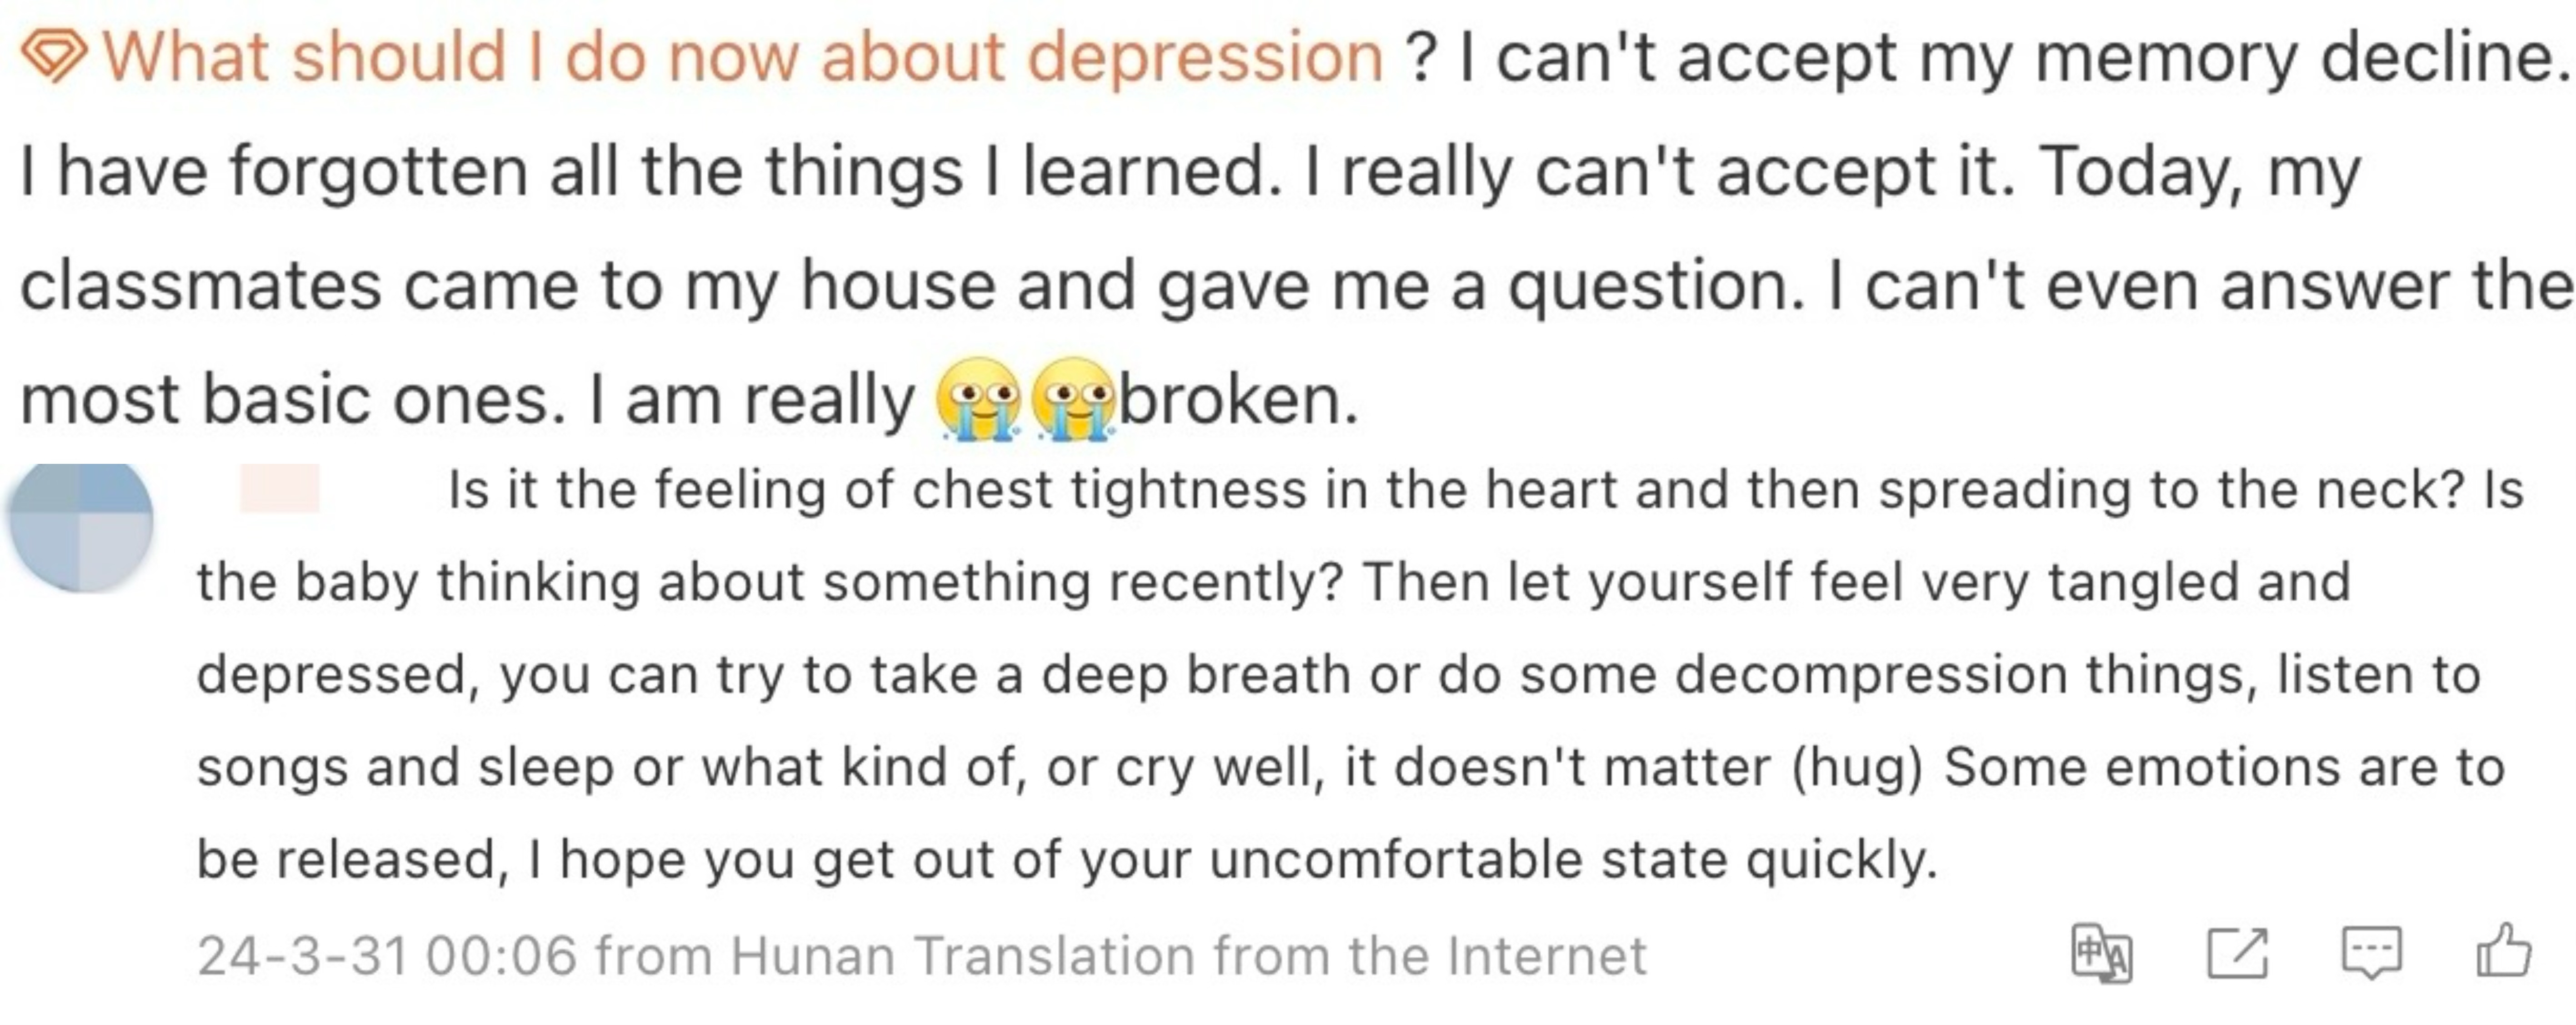
\includegraphics[width=1\columnwidth]{images/postreplyy.jpeg}
    \caption{Example of user post and reply.}
    \label{fig:cases_post_reply}
\end{figure}


We first manually annotated 1000 posts and replies according to the categories in \tabref{tab:Post_category} and then used the PaddleNLP~\footnote{\url{https://github.com/PaddlePaddle/PaddleNLP}} multi-label classification model to classify the post and reply content. The F1-score for multiple classifiers in the post categories is 80.6\%, and the F1-score for multiple classifiers in the reply categories is 62.8\%. Details of the multi-label classification experiment can be found in Appendix \ref{apd:classify_details}. 
%\SY{briefly show the classification accuracy here.} 

%\KZ{Why did you classify the posts and replies like this? Is there %any theretical basis, or is it purely by observation?
%If it's by observation, what's the size of your observation?}



\subsection{Depressed User Identification} 
\label{sec:depression_detection}
Once we have collected the data from Weibo, the next step is to identify depressed users who need help. Since not all users in the Weibo Depression Super Topic Community suffer from depression, we perform a process called depression detection to find the depressed users.
%\KZ{There's no such thing called ``depression users'', it should be ``depressed users''.}
Following ~\citet{zhang2022symptom}, which predicted whether users suffer from multiple mental disorders on social media through their posting history, we utilized a BERT model \cite{devlin2018bert} to train the classifier for depression detection. Specific implementation details can be found in the Appendix~\ref{apd:dd_details}.
%\KZ{Depending on your space constraint, some details
%can be moved back here.}
\begin{figure*}[th]
	\centering
	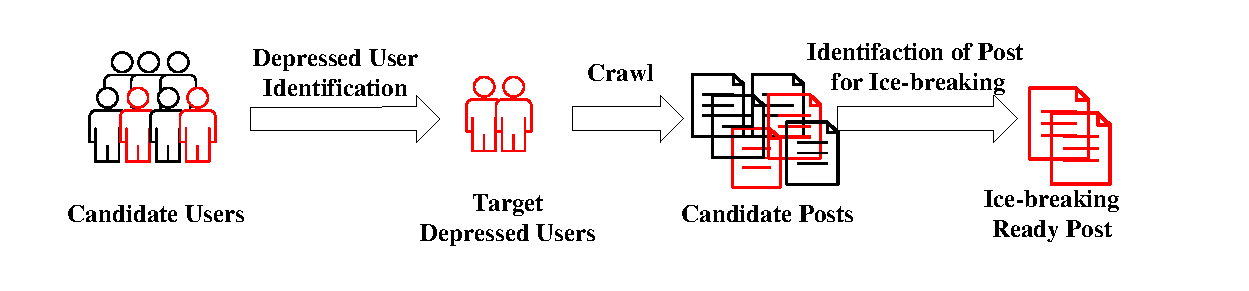
\includegraphics[width=1.7\columnwidth]{images/pipeline1.pdf}
	\caption{\ZT{The pipeline used to find target depressed users and posts.}}
\label{fig:pipeline1}
\end{figure*}

\subsection{``Three-Round Interaction''}
\label{sec:3round}
As \figref{fig:pipeline2} shows, the ``Three-Round Interaction'' involves users posting (first round), our robot commenting on the post (second round), and depressed users replying to our comments (third round).
We focus only on the ``three-round interaction'' between the user’s post and replies, because it is sufficient to evaluate whether we successfully initiated the interaction and broke the ice. 
During this process, we first identify the ice-breaking point, then generate an icebreaker, and finally analyze the user's replies. The details of this interaction process will be introduced in the following part.

\begin{figure}[th]
	\centering
	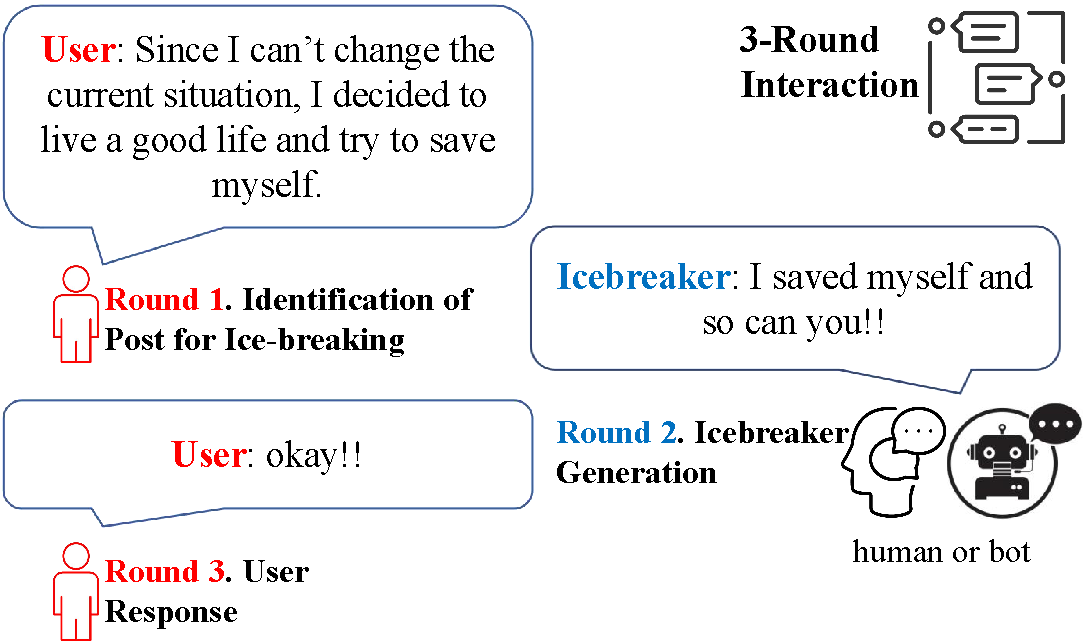
\includegraphics[width=1\columnwidth]{images/pipeline2.pdf}
	\caption{\ZT{An example of ``three-round interaction'' with users.}}
 %\KZ{The words in the pic should correspond to the Round x text below.}
\label{fig:pipeline2}
\end{figure}
%\KZ{At this point you should discuss what is three-round interaction and why it's important here.
%We don't want to go beyond three round because that's all we need to do ice-breaking, and we leave the rest
%to the other chatbots. Only after you talk about three-round %interaction, then you talk about to to carry out
%this interaction, which includes ice-breaking point id, and icebreaker generation, and reply analysis.}

\paragraph{Round 1: Identification of Post for Ice-breaking}
\label{sec:IBP}
Some depressed users post solely to express their emotions and prefer not to engage in communication with others. Therefore, our objective is to identify those depressed users who are willing to engage in conversations and pinpoint suitable posts where we can proactively initiate an icebreaker. By observing the posts of depressed users, and their responses, we can determine the 
ice-breaking point of a user. For instance, if a stranger comments on a depressed user's post and receives a response from the user, it indicates that this is a situation in which the user is open to ice-breaking.
The identification criteria for ice-breaking points are as follows:
\begin{enumerate}
	%\item The number of comments on a certain post is greater than 1.
	%\item The ID of a depressed user has appeared under this post.
    %\item The commenting user must be a stranger to the depressed user.  We define a stranger as a user whose ID has not appeared in the depressed user's posting history, including likes, replies, and reposts, nor has the depressed user's ID appeared in the commenting user's history.  Additionally, neither the commenting user nor the depressed user can be each other's followers or followees.
    %\KZ{In order to prove that this commentor is a stranger, not only he has never commented on the depressed user before, the depressed user has also never commented on his posts before, right?}
    \item \ZT{A post serving as an ice-breaking point must be a recent post from a depressed user, such as within one week.}
    \item \ZT{The post must have at least one comment from a stranger.} We define a stranger as a user whose ID has not appeared in the depressed user's posting history, including likes, replies, and reposts, nor has the depressed user's ID appeared in the commenting user's history.  Additionally, neither the commenting user nor the depressed user can be each other's followers or followees.
    \item \ZT{The depressed user who made the post has replied to the stranger's comment.}
\end{enumerate}

\paragraph{Round 2: Icebreaker Generation}
After identifying depressed users and posts to initiate icebreakers, we must select appropriate ice-breaking strategies based on different post categories. We will exclude the fifth reply category (Discouraging reply) in \secref{sec:category} since it is not conducive to the 
relief of depressed users. All other four categories, including emotional support and resonance, suggestions and solutions, emotional talk and communication and encouragement and affirmation, will be the
candidates of our ice-breaking strategy. 

For the chatbot's reply, we combined the four strategies mentioned above to form a prompt for chatGPT to automatically generate an icebreaker.More details on the automatic generation of icebreakers can be found in Appendix~\ref{apd:icebreaker_ge}.
%Next we will experiment with these strategies to see their effects.
%\KZ{Are you going to include the different %strategies here? Otherwise
%this subsection is too brief.}
%\KZ{I think here we should talk about different role's setup and camouflagging (how we maintain our bot's personal profile
%etc. This is quite interesting. But it could be accused on cheating the user. But for science, I think it's ok. So we need to discuss the legality of this a bit in the Ethics section.}

\paragraph{Round 3: User Response}
When both chatbots and humans engage in two-round of conversations with depressed users, we need to count the responses from depressed users to verify the effectiveness of our ice-breaking.